
\documentclass[a4paper,12pt, oneside]{book}

%  Русский язык
\usepackage{cmap}					% Улучшенный поиск русских слов
\usepackage[T2A]{fontenc}			% кодировка
\usepackage[utf8]{inputenc}			% кодировка исходного текста
\usepackage[english,russian]{babel}	% локализация и переносы
\usepackage{pscyr}					% нормальные шрифты

% Колонтитулы
\usepackage{fancybox,fancyhdr}
\usepackage{lastpage}
\fancyhf{}
\fancypagestyle{all}
{
	\fancyhead{}
	\fancyhead[C]{\vspace{-5mm}Контрольная работа 12 Вариант Попов Юрий СКБ-171\vspace{3mm}}
	\fancyfoot{}
	\fancyfoot[C]{\hfill  \thepage  \hfill}
}

% Картинки и графики
\usepackage{wrapfig}
\usepackage{pgfplots}
\pgfplotsset{compat=1.9}

% Ссылки
\usepackage{xcolor}
\usepackage{color,colortbl} % раскраска таблиц
\usepackage[unicode, pdftex]{hyperref}
\definecolor{linkcolor}{HTML}{000000} 	% цвет ссылок
\definecolor{urlcolor}{HTML}{8B000F}	% цвет гиперссылок
\hypersetup{urlcolor=urlcolor, linkcolor=linkcolor, colorlinks=true}

% Размеры
\setlength{\paperwidth}{210mm}
\setlength{\paperheight}{297mm}
\setlength{\textheight}{225mm} 			% высота без колонтитулов
\setlength{\textwidth}{170mm}			% ширина текста
\oddsidemargin=0pt
\setlength{\headheight}{2mm}			% высота колонтитула
\setlength{\headsep}{5mm} 	% от блока текста до верхнего колонтитула
\setlength{\footskip}{10mm}  % от блока текста до нижнего колонтитула

% Математика
\usepackage{amsmath,amsfonts,amssymb,amsthm,mathtools,mathtext} 
\usepackage{latexsym,array,epsfig,wasysym}
\usepackage[all]{xy}
\let\int\varint
\def\Int{\int\limits}
\def\IInt{\iint\limits}
\def\IIInt{\iiint\limits}
\DeclarePairedDelimiter\floor{\lfloor}{\rfloor}


% Оглавление 
\usepackage{setspace}

\usepackage{tocloft} %регулировка расположения TableOfContent (Оглавления) на странице

%\setcounter{tocdepth}{1} % отменяет вывод в оглавление subsection and subsubsection
%\setcounter{secnumdepth}{1} %отменяет номерацию секций в тексте и оглавлении.
\usepackage{tocloft} %регулировка расположения TableOfContent (Оглавления) на странице

\renewcommand{\cfttoctitlefont}{\hspace{0.38\textwidth} \bfseries\MakeUppercase} %уменьшаем размер шрифта и ровняем по центру

% % Межстрочные отступы в Оглавлении:
\setlength{\cftbeforetoctitleskip}{5mm} %отступ Оглавления от верхнего поля страницы.
\setlength{\cftbeforechapskip}{14mm} %отступ между главами
\setlength{\cftbeforesecskip}{5mm} %отступ между секциями \section{title}

% % Отступы от левого поля:
\setlength{\cftchapindent}{1mm} %отступ между левым полем и \chapter{}
\setlength{\cftsecindent}{13mm} %отступ между левым полем и \section{title}

% % Отточия в Оглавлении
\renewcommand\cftchapdotsep{\cftdot} %добавляет отточия после \chapter{title}
%\renewcommand{\cftchapleader}{\cftdotfill{\cftchapdotsep}} %делает отточия после \chapter{title} тонкими, (по умолчанию жирные).
\renewcommand\cftsecdotsep{\cftdot} %делает отточия после \section{title} частыми.

% % Интервалы между абзацами, главами и так далее:
\usepackage{titlesec}

\titleformat{\chapter}[display]
{\filcenter}
{\MakeUppercase{\chaptertitlename} \thechapter}
{8pt}
{\bfseries}{}

\titleformat{\section}
{\normalsize\bfseries}
{\thesection}
{1em}{}

\titleformat{\subsection}
{\normalsize\bfseries}
{\thesubsection}
{1em}{}

% Настройка вертикальных и горизонтальных отступов
\titlespacing*{\chapter}{0pt}{-30pt}{8pt}
\titlespacing*{\section}{\parindent}{*4}{*4}
\titlespacing*{\subsection}{\parindent}{*4}{*4}


\begin{document} % начало документа	
	\pagestyle{plain}
	
	\begin{titlepage}	
		\begin{center}
			{\Huge \textbf{Математическая статистика}}
			\vspace{30mm}
			
			{\Huge Домашняя работа № 4 \\}
			\vspace{30mm}
			
			{\huge Проверка статистических гипотез}
			\vspace{30mm}
			
			{\Large Попов Юрий, СКБ-172}
		\end{center}
	\end{titlepage}
	
	
	
	\begin{spacing}{0.99}          
		\tableofcontents %Оглавление. Корректно создается за два прогона tex файла.               
	\end{spacing}

\newpage
\begin{center}
	{\Huge{\bf{Предисловие}}}
\end{center}


%-------------------------------------Предислов

\setcounter{secnumdepth}{-1} % убираем нумерацию 


%-------------------------------------Предисловие
\newpage

\begin{center}
	\textbf{\Large Немного теории}
\end{center}

\normalsize{\textbf{Определение 1}} \textit{ Статистическая гипотеза } - это некоторое предположение о виде или параметрах распределений\\

\normalsize{\textbf{Определение 2}} \textit{ Статистический критерий  } - это правило, по которому каждой реализации выборки ставится в соответствие решение: принимаем гипотезу $ H_0 $ или отвергаем ее( то есть принимаем гипотезу $ H_1 $)\\

\normalsize{\textbf{Определение 3}} \textit{ Уровень значимости статистического теста } - допустимая для данной задачи вероятность ошибки первого рода, то есть вероятность отклонить нулевую гипотезу, когда на самом деле она верна\\

\normalsize{\textbf{Определение 4}} В случае, когда $ H_0 $ и $ H_1 $ - простые гипотезы, $ P(x \in \mathcal{X} | H_0)) = \lambda $ - {\it ошибка 1 рода}

$ \beta = P(H_0 | H_1) $ - \textit{ошибка второго рода}\\

\normalsize{\textbf{Определение 5}} Если $ H_0 $ состоит из одного определения, то говорят, что $ H_0 $ - \textit{простая гипотеза}, иначе $ H_0 $  \textit{сложная гипотеза}\\

\normalsize{\textbf{Определение 6}} Если $ H_1 $ состоит из одного определения, то говорят, что $ H_1 $ - \textit{простая гипотеза}, иначе $ H_1 $  \textit{сложная гипотеза}\\

\newpage
\begin{center}
	\textbf{\Large Перейдем к практике}
\end{center}

\chapter{4.1 Геометрическое распределение}

В качестве критерия я взял критерий Пирсона. Этот метод позволяет оценить статистическую значимость различий двух или нескольких относительных показателей. Это наиболее часто употребляемый критерий для проверки гипотезы о принадлежности наблюдаемой выборки некоторому теоретическому закону распределения.

Этот критерий универсальный

Для каждой выборки составим расчетную таблицу:

\begin{figure}[h!]
	\begin{center}
		\begin{minipage}[h]{0.47\linewidth}
			\center{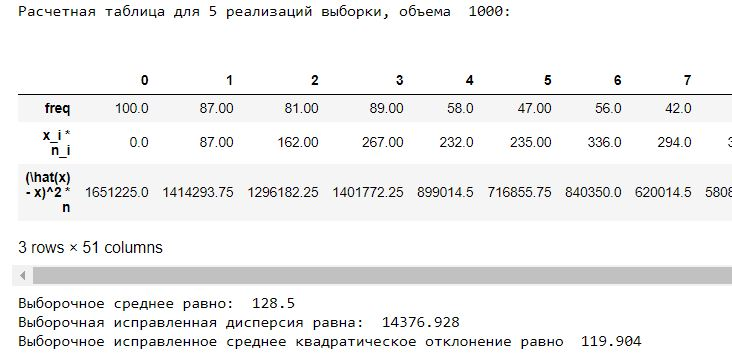
\includegraphics[width=1\linewidth]{fotos/geom/r1}} \\
		\end{minipage}
		\hfill
		\begin{minipage}[h]{0.47\linewidth}
			\center{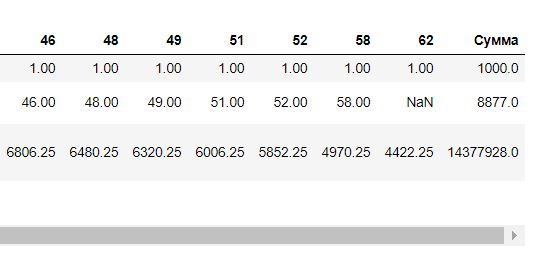
\includegraphics[width=1\linewidth]{fotos/geom/r1_2}}\\
		\end{minipage}
		\hfill
		\begin{minipage}[h]{0.47\linewidth}
			\center{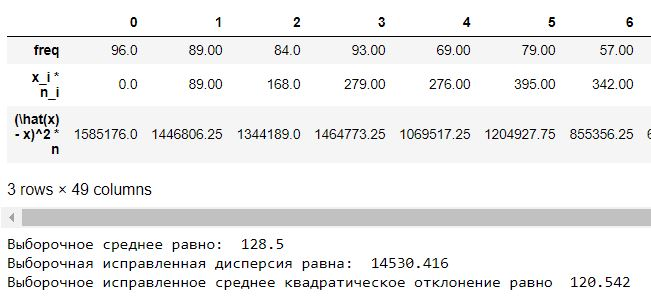
\includegraphics[width=1\linewidth]{fotos/geom/r2}}\\
		\end{minipage}
		\hfill
		\begin{minipage}[h]{0.47\linewidth}
			\center{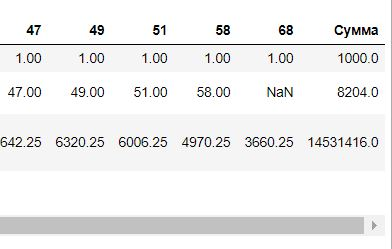
\includegraphics[width=1\linewidth]{fotos/geom/r2_2}}\\
		\end{minipage}
		\hfill	
		\begin{minipage}[h]{0.47\linewidth}
			\center{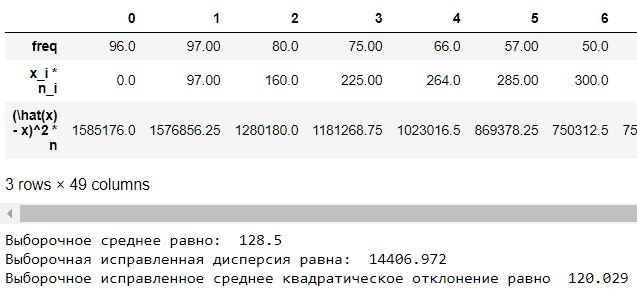
\includegraphics[width=1\linewidth]{fotos/geom/r3}}\\
		\end{minipage}
		\hfill
		\begin{minipage}[h]{0.47\linewidth}
			\center{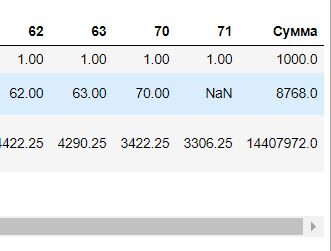
\includegraphics[width=1\linewidth]{fotos/geom/r3_3}}\\
		\end{minipage}
	\end{center}
\end{figure}

		
\begin{figure}[h!]
	\begin{center}
		\begin{minipage}[h]{0.47\linewidth}
			\center{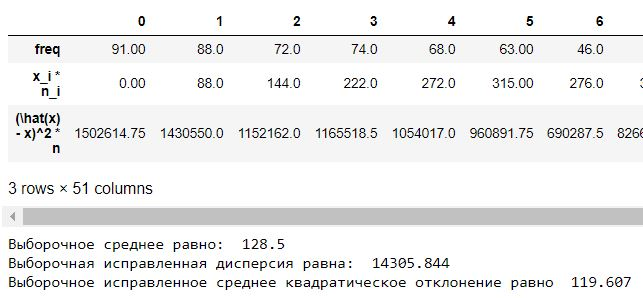
\includegraphics[width=1\linewidth]{fotos/geom/r4}}\\
		\end{minipage}
		\hfill	
		\begin{minipage}[h]{0.47\linewidth}
			\center{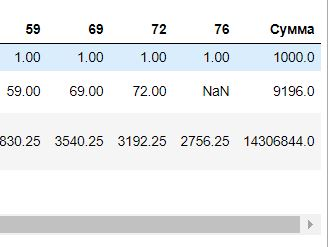
\includegraphics[width=1\linewidth]{fotos/geom/r4_4}}\\
		\end{minipage}
		\hfill
		\begin{minipage}[h]{0.47\linewidth}
			\center{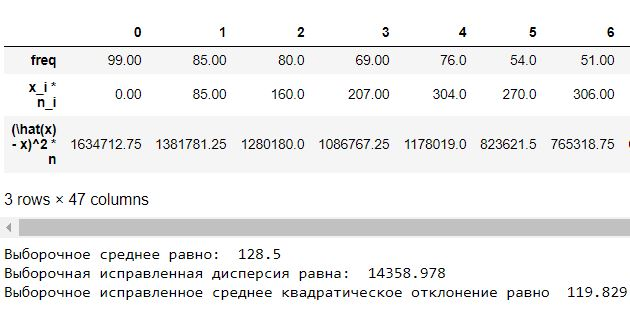
\includegraphics[width=1\linewidth]{fotos/geom/r5}}\\
		\end{minipage}
		\hfill
		\begin{minipage}[h]{0.47\linewidth}
			\center{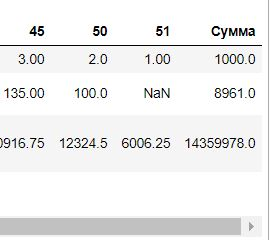
\includegraphics[width=1\linewidth]{fotos/geom/r5_5}}\\
		\end{minipage}
	\end{center}
\end{figure}


Выдвинем гипотезу $ H_0 $: распределение генеральной совокупности $ X $ подчинено геометрическому закону с параметром p Проверим эту гипотезу по критерию Пирсона при уровне значимости $ \lambda  = 0.05 $






\newpage
\chapter{4.2 Экспоненциальное распределение}




\begin{thebibliography}{99}
	\bibitem{rt1} 
	\bibitem{rt2} \href{https://towardsdatascience.com/what-is-exponential-distribution-7bdd08590e2a}{ссылка1}
	\bibitem{rt3}  \href{https://www.statisticshowto.datasciencecentral.com/exponential-distribution/}{ссылка2}
	\bibitem{rt4}  // \href{http://www.ams.jhu.edu/~dan/550.435/notes/COURSENOTES435.pdf}{ссылка3}
	\bibitem{rt5}  // \href{http://www.obzh.ru/nad/4-3.html}{ссылка4}
\end{thebibliography}

\end{document}
